\documentclass{article}
\usepackage{eecstex}
\usepackage{physics}
\usepackage{pgfplots}

\renewcommand{\thesubsection}{\thesection.\arabic{subsection}}
\renewcommand{\thesubsubsection}{\thesubsection.\alph{subsubsection}}
\renewcommand{\labelenumi}{\arabic{enumi}.}
\newcommand{\F}{\mathcal{F}}
\newcommand{\sinc}{\operatorname{sinc}}
\newcommand{\rect}{\operatorname{rect}}

\title{EE 120 HW 07}
\author{Bryan Ngo}
\date{2021-03-10}

\begin{document}

\maketitle

\section{CTFT Properties}

\subsection{}

\begin{align}
    \F\{e^{-at} \cos(\omega_0 t) u(t)\} = \frac{1}{2\pi} \F\{e^{-at} u(t)\} \ast \F\{\cos(\omega_0 t)\} &= \frac{1}{4\pi} \qty(\frac{1}{a + j \omega}) \ast \qty(\delta\qty(\omega - \frac{\omega_0}{2\pi}) + \delta\qty(\omega + \frac{\omega_0}{2\pi})) \\
    &= \frac{1}{4\pi} \qty(\frac{1}{a + j \qty(\omega - \frac{\omega_0}{2\pi})} + \frac{1}{a + j \qty(\omega + \frac{\omega_0}{2\pi})})
\end{align}

\subsection{}

\begin{align}
    \F\{e^{-2 |t|} \sin(3t)\} &= \int_{\R} e^{-2 |t|} \sin(3t) e^{-j \omega t} \, dt \\
    &= 2 \int_0^\infty e^{-2t} \sin(3t) e^{-j \omega t} \, dt = 2\F\{e^{-2t} \sin(3t) u(t)\} \\
    &= \frac{1}{\pi} \F\{e^{-2t} u(t)\} \ast \F\{\sin(3t)\} \\
    &= \frac{1}{2\pi j} \qty(\frac{1}{2 + j \omega}) \ast \qty(\delta\qty(\omega - \frac{3}{2\pi}) + \delta\qty(\omega + \frac{3}{2\pi})) \\
    &= \frac{1}{2\pi j} \qty(\frac{1}{2 + j \qty(\omega - \frac{3}{2\pi})} + \frac{1}{a + j \qty(\omega + \frac{3}{2\pi})})
\end{align}

\subsection{}

\begin{align}
    \F\qty{\qty(\frac{\sin(\pi t)}{t}) \ast \qty(\frac{\sin(2\pi t)}{t})} &= \pi \F\{\sinc(t) \ast 2 \sinc(2\pi t)\} \\
    &= \pi \F\{\sinc(t)\} \cdot 2 \F\{\sinc(2\pi t)\} \\
    &= \pi \rect(\omega) \cdot \frac{2}{2\pi} \rect\qty(\frac{\omega}{2\pi}) = \rect(\omega) \rect\qty(\frac{\omega}{2\pi})
\end{align}

\section{2nd Order LCCDE}

\begin{equation}
    \dv[2]{y(t)}{t} + 2\dv{y(t)}{t} + 3 y(t) = 4\dv{x(t)}{t} - x(t)
\end{equation}

\subsection{}

Finding the frequency response \(y(t) = e^{j \omega t}\),
\begin{equation}
    -\omega^2 e^{j \omega t} + 2j \omega e^{j \omega t} + 3 e^{j \omega t} = \underbrace{(3 - 2j - \omega^2)}_{A(\omega)} e^{j \omega t}
\end{equation}
By the eigenfunction property, \(A(\omega) = 3 - 2j \omega - \omega^2\).

\subsection{}

Finding the frequency response \(x(t) = e^{j \omega t}\),
\begin{equation}
    4j \omega e^{j \omega t} - e^{j \omega t} = \underbrace{(4j \omega - 1)}_{B(\omega)} e^{j \omega t}
\end{equation}
By the eigenfunction property, \(B(\omega) = 4j \omega - 1\).

\subsection{}

Setting the two equal to each other gives us that \(H(\omega) = \frac{B(\omega)}{A(\omega)} = \frac{4j \omega - 1}{3 - 2j - \omega^2}\).

\section{A Fourier System}

\begin{align}
    \F\{x(t)\} &= 2\pi X(-t) \\
    \F^2\{x(t)\} &= \F\{2\pi X(-t)\} = 4\pi^2 X(-t) \\
    \F^3\{x(t)\} &= \F\{4\pi^2 X(-t)\} = 8\pi^3 X(-t) = w(t)
\end{align}

\section{DTFS as a Linear Operation}

\subsection{}

\begin{equation}
    x[n] = \sum_{k \in [0, N - 1]} a_k e^{j k \omega_0 n} \implies
    \begin{bmatrix}
        x[0] \\
        x[1] \\
        x[2] \\
        \vdots \\
        x[N - 1]
    \end{bmatrix}
    =
    \underbrace{\begin{bmatrix}
        1 & 1 & 1 & \cdots & 1 \\
        1 & e^{j \omega_0} & e^{j \omega_0 2} & \cdots & e^{j \omega_o (N - 1)} \\
        1 & e^{j \omega_0 2} & e^{j \omega_0 4} & \cdots & e^{j \omega_o 2(N - 1)} \\
        \vdots & \vdots & \vdots & \ddots & \vdots \\
        1 & e^{j \omega_0 (N - 1)} & e^{j \omega_0 2(N - 1)} & \cdots & e^{j \omega_0 (N - 1) (N - 1)}
    \end{bmatrix}}_{\mathcal{W}}
    \begin{bmatrix}
        a_0 \\
        a_1 \\
        a_2 \\
        \vdots \\
        a_{N - 1}    
    \end{bmatrix}
\end{equation}

\subsection{}

\begin{align}
    \begin{bmatrix}
        1 \\
        0 \\
        0 \\
    \end{bmatrix}
    &=
    \begin{bmatrix}
        1 & 1 & 1 \\
        1 & e^{j \frac{2\pi}{3}} & e^{j \frac{4\pi}{3}} \\
        1 & e^{j \frac{4\pi}{3}} & e^{j \frac{8\pi}{3}}
    \end{bmatrix}
    \begin{bmatrix}
        a_0 \\
        a_1 \\
        a_2
    \end{bmatrix} \\
    \implies \begin{bmatrix}
        a_0 \\
        a_1 \\
        a_2
    \end{bmatrix}
    &= 
    \begin{bmatrix}
        1 & 1 & 1 \\
        1 & e^{j \frac{2\pi}{3}} & e^{j \frac{4\pi}{3}} \\
        1 & e^{j \frac{4\pi}{3}} & e^{j \frac{8\pi}{3}}
    \end{bmatrix}^{-1}
    \begin{bmatrix}
        1 \\
        0 \\
        0
    \end{bmatrix}
    =
    \begin{bmatrix}
        1 / 3 \\
        1 / 3 \\
        1 / 3 \\
    \end{bmatrix}
\end{align}

\subsection{}

\begin{align}
    a_k &= \frac{1}{N} \sum_{n \in [0, N - 1]} x[n] e^{-j k \omega_0 n} \\
    \implies
    \begin{bmatrix}
        a_0 \\
        a_1 \\
        a_2 \\
        \vdots \\
        a_{N - 1}    
    \end{bmatrix}
    &=
    \underbrace{\frac{1}{N} \begin{bmatrix}
        1 & 1 & 1 & \cdots & 1 \\
        1 & e^{-j \omega_0} & e^{-j \omega_0 2} & \cdots & e^{-j \omega_o (N - 1)} \\
        1 & e^{-j \omega_0 2} & e^{-j \omega_0 4} & \cdots & e^{-j \omega_o 2(N - 1)} \\
        \vdots & \vdots & \vdots & \ddots & \vdots \\
        1 & e^{-j \omega_0 (N - 1)} & e^{-j \omega_0 2(N - 1)} & \cdots & e^{-j \omega_0 (N - 1) (N - 1)}
    \end{bmatrix}}_{\mathcal{W}^{-1}}
    \begin{bmatrix}
        x[0] \\
        x[1] \\
        x[2] \\
        \vdots \\
        x[N - 1]
    \end{bmatrix}
\end{align}

\subsection{}

\begin{equation}
    \frac{1}{3}
    \begin{bmatrix}
        1 & 1 & 1 \\
        1 & e^{j \frac{2\pi}{3}} & e^{j \frac{4\pi}{3}} \\
        1 & e^{j \frac{4\pi}{3}} & e^{j \frac{8\pi}{3}}
    \end{bmatrix}
    \begin{bmatrix}
        1 & 1 & 1 \\
        1 & e^{-j \frac{2\pi}{3}} & e^{-j \frac{4\pi}{3}} \\
        1 & e^{-j \frac{4\pi}{3}} & e^{-j \frac{8\pi}{3}}
    \end{bmatrix}
    =
    \frac{1}{3} \begin{bmatrix}
        3 & 0 & 0 \\
        0 & 3 & 0 \\
        0 & 0 & 3
    \end{bmatrix} = \bm{I}_3
\end{equation}

\section{Derivatives of a Signal}

\subsection{}

\begin{equation}
    \dv[k]{t} (h \ast x)(t) = \dv[k]{t} \int_{\R} x(\tau) h(t - \tau) \, d\tau = \int_{\R} x(\tau) \pdv[k]{t} h(t - \tau) \, d\tau = \qty(\underbrace{\dv[k]{t} h}_{h_k} \ast x)(t)
\end{equation}

\subsection{}

\begin{align}
    h_1(t) &= -\frac{t}{\sqrt{2\pi}} e^{-\frac{t^2}{2}} \\
    H_1(\omega) &= \F\qty{-\frac{t}{\sqrt{2\pi}} e^{-\frac{t^2}{2}}} = -j \F\qty{-jt \frac{1}{\sqrt{2\pi}} e^{-\frac{t^2}{2}}} = -j \dv{\omega} H(\omega) \\
    H(\omega) &= \F\qty{\frac{1}{\sqrt{2\pi}} e^{-\frac{t^2}{2}}} = \frac{1}{\sqrt{2\pi}} \F\qty{e^{-\qty(\frac{t}{\sqrt{2}})^2}} = \frac{\sqrt{2}}{\sqrt{2\pi}} \sqrt{\pi} e^{-\frac{\omega^2}{2}} = e^{-\frac{\omega^2}{2}} \\
    \implies H_1(\omega) &= -j \dv{\omega} H(\omega) = j\omega e^{-\frac{\omega^2}{2}}
\end{align}
\begin{center}
    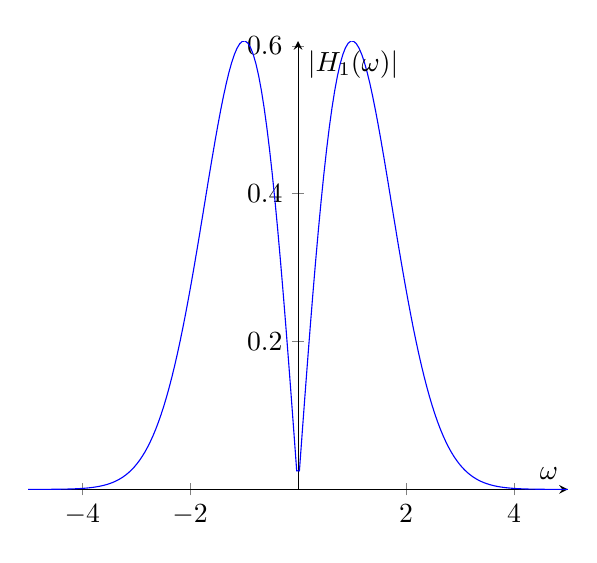
\begin{tikzpicture}
        \begin{axis}[
            xlabel=\(\omega\), ylabel={\(|H_1(\omega)|\)},
            axis lines=middle,
        ]
        \addplot[
            color=blue,
            domain=-5:5,
            samples=200
        ]{abs(x*exp(-x^2/2))};
        \end{axis}
    \end{tikzpicture}
\end{center}

\subsection{}

\begin{equation}
    y(t) = \dv{t} e^{j \omega t} = j\omega e^{j \omega t} \implies |H_d(\omega)| = \omega
\end{equation}
We find that \(\frac{|H_1(omega)|}{|H_d(\omega)|} = e^{-\frac{\omega^2}{2}}\), so this means that this signal isnot attenuated through this filter of the ratio, so it is amplified.

\end{document}
